%-------------------------------------------------------------------------------
\section{Why}\label{s:why}
%-------------------------------------------------------------------------------


The immediately relevant question that falls out of this observed poor behavior
is how fundamental it is: does Linux operate at a timescale and fidelity that is
fundamentally unable to do a better job of isolating these processes, or, if
not, why is it unable isolate currently?

Linux' preemption granularity is that of hardware ticks, which is usually 4ms
(including in this experiment), and at minimum 1ms. Related work that focuses on
isolating LC processes from BE antagonists, by contrast, makes a scheduling
decision every 10 $\mu$s~\cite{TODO}. This can become a problem when coupled
with Linux's weighted fair share scheduler: when a BE process gets the CPU, as
even with a very low weight it occasionally should, it will then run for a full
tick (barring any intermediate interrupts).

However, a closer look shows that this cannot be the problem, or at least not
the full problem. 

The first reason has to do with the fact that Linux's scheduler approximates
weighted fair share scheduling: it estimates the time a process should have
gotten and compares it with how much it got, and schedules the process owed the
most time. Thus, even though it does not have the ability to interrupt the BE
process exactly at the moment that it ran over the cputime it should have
gotten, once the tick the BE ran for is over the scheduler will account for the
fact that the process got more time than it should have, and that will push back
when it is scheduled next.\hmng{show schedviz of this happening?} 

A second reason why this can't be the whole problem is that if those 4ms were
the problem, we would expect the experiment to show bursts in which LC latency
spikes while the BE is running, and then a stabilization when BE doesn't; but
instead we see a consistent impact on the LC latency.

Finally, the latency impact is disproportionate. Certainly a very large number
of low-weight processes could add up to a significant weight in the system, for
example if a machine has 10000 BE workloads with weight 1, and one LC workload
with weight 10000, the LC would in expectation get half the machine. However, in
this experiment, we only started two BE tasks, each with weight 1. Even if
mulitplied by a factor of 4ms, the order of magnitude is off.

In fact what is actually happening is not poor scheduling within a single core,
but across cores. Linux maintains a separate runqueue on each core, in order to
avoid the synchronization overheads of accessing global state for every
scheduling decision. Within each runqueue, Linux does a pretty good job of
maintaining the correct ratio of received cputime. This is modulo the
aforementioned effects of the 4ms tick granularity, but over longer periods of
time it enforces the expected split.

However, the per-core runqueues mean that the weight is only strictly enforced
within the individual runqueues, \ie{} within each core. This leads to a failure
mode, which is that it can occur that \textit{one core is running a BE process,
while an LC process is waiting on another}. This can happen as follows: suppose
there are two cores, each with some LC threads blocked on sockets and some
running cpu-bound BE threads. If three requests come in, then two will be placed
on one core and one on the other. Once the core with the one request finishes
processing it, it will see no further high-weight queued processes and resume
running the BE thread, completely unaware that at a different core there is a
queued and waiting high-weight thread. In an alternative world where there is no
BE thread waiting, the core will try to steal work before going completely into
an idle state, and in doing so would steal the queued LC thread.

\begin{figure}[t]
    \centering
    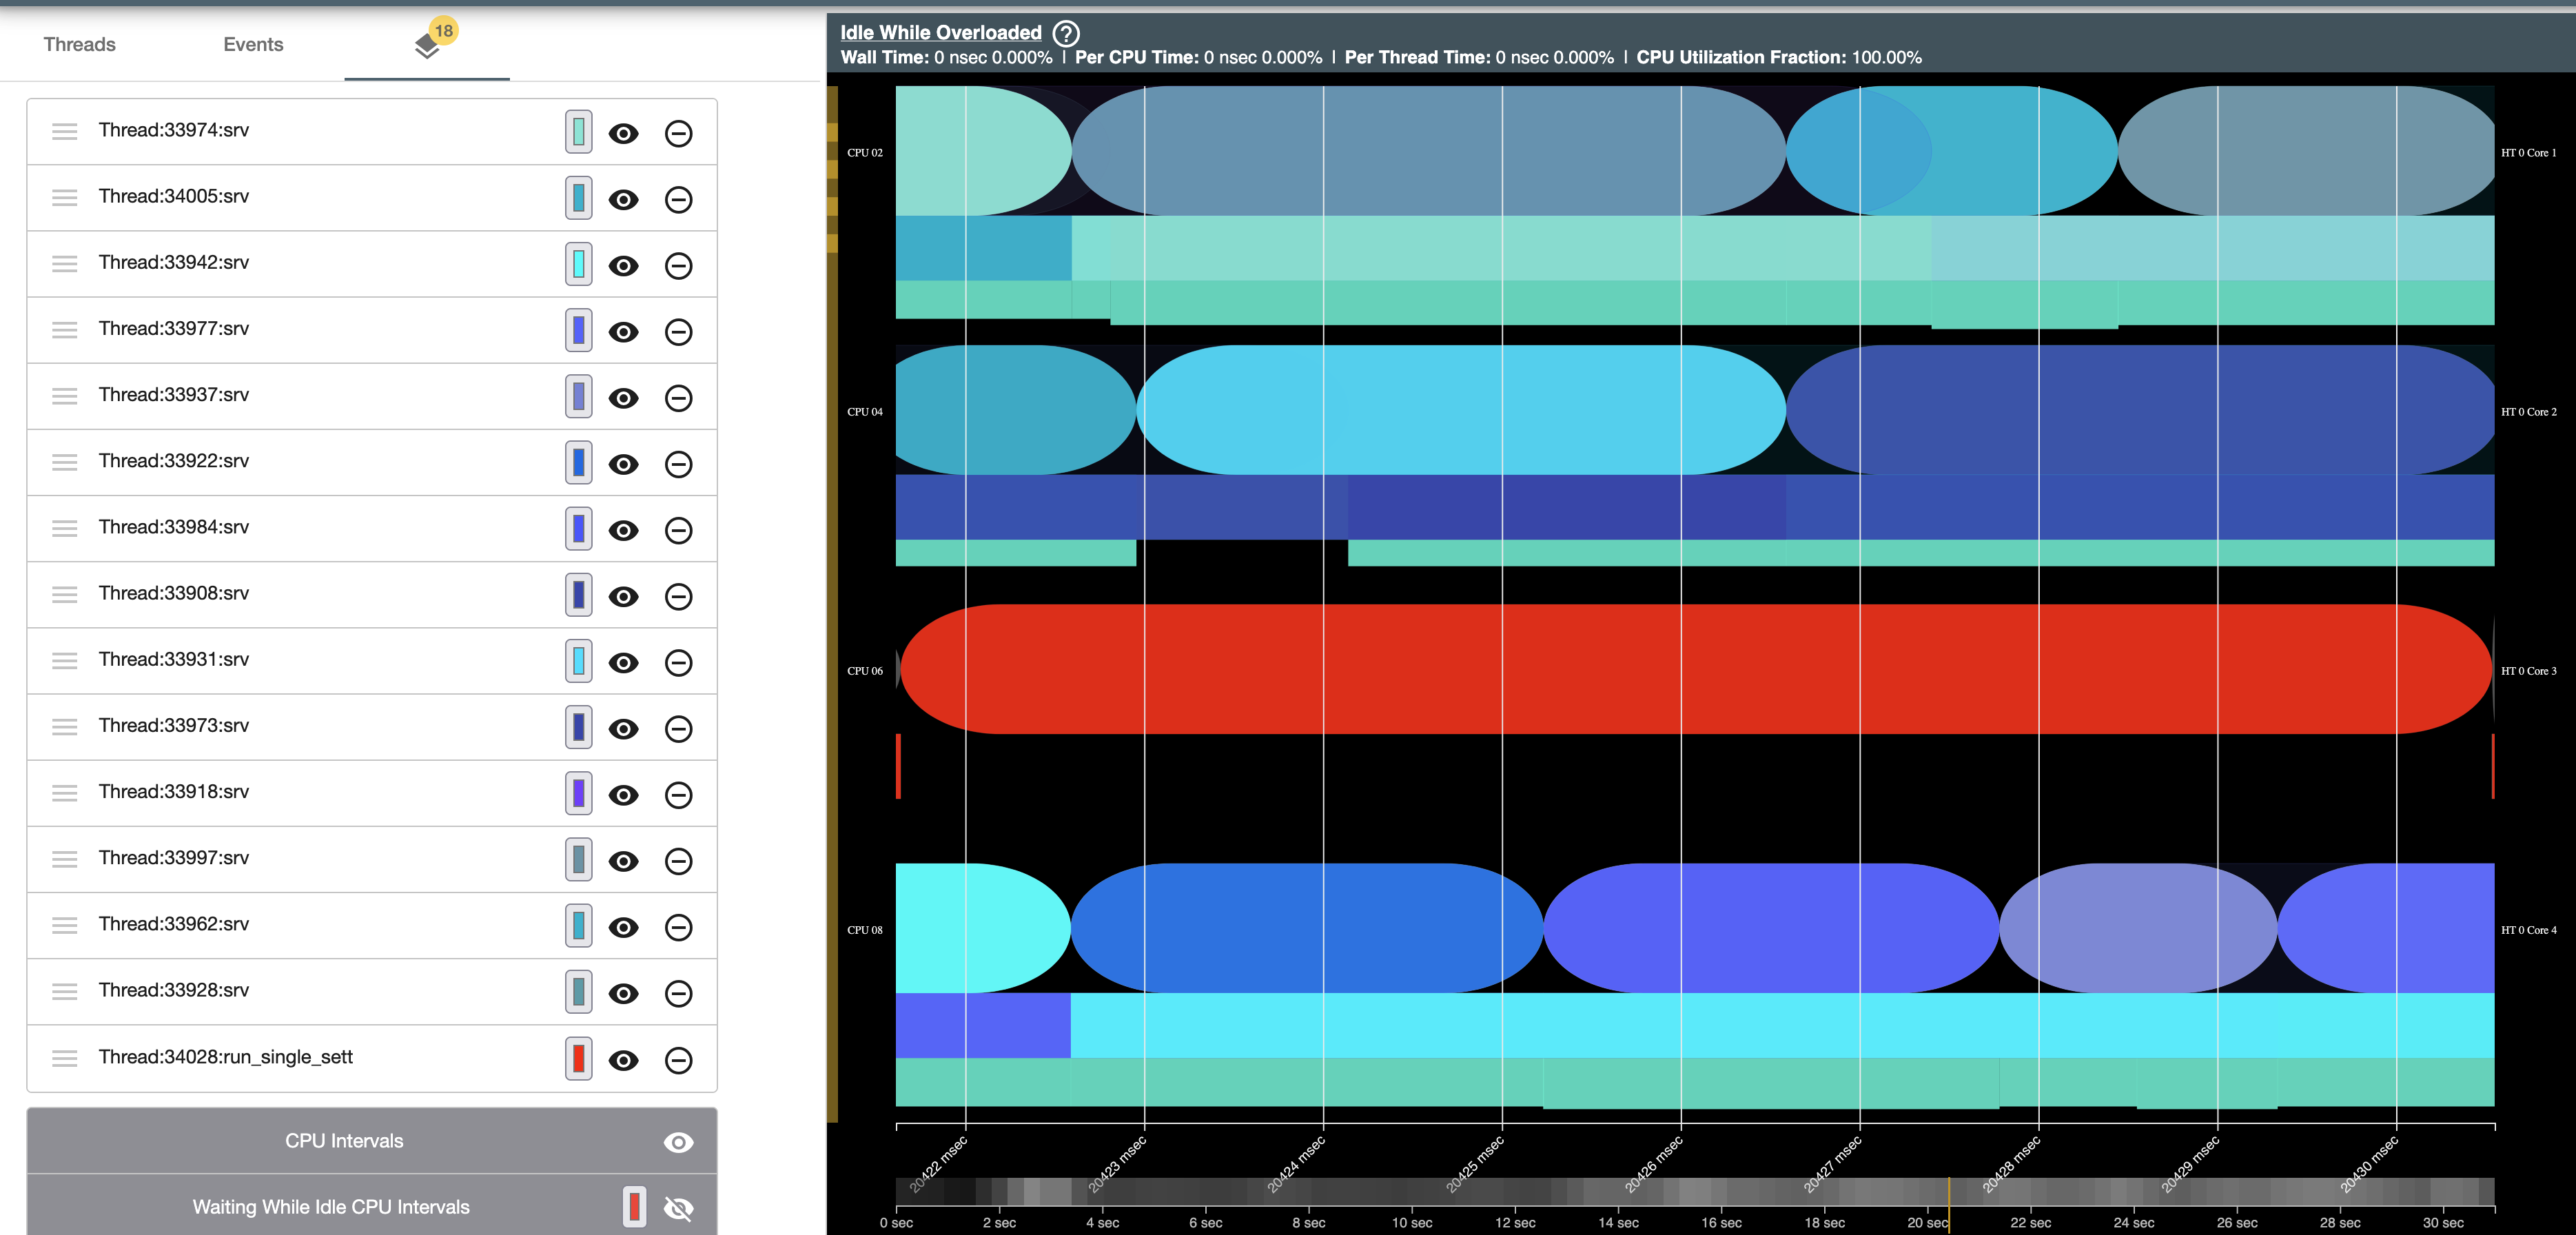
\includegraphics[width=\columnwidth]{graphs/schedviz.png}
    \caption{Each thread is a different color. Circles represent which
    thread is running on that core, while rectangles underneath show waiting but
    runnable threads. Core numbers are 2,4,6,8 because this was run on a NUMA
    node so those are the cores that are closest to each other
    }\label{fig:schedviz}
\end{figure}

In fact, we see this occurring in traces of the experiment in
\autoref{fig:unedited-weight}. We examine the trace using schedviz~\cite{TODO},
a tool that visualizes perf traces. A 10ms outtake of the resulting image is
show in \autoref{fig:schedviz}. This shows the explained phenomenon occurring:
on core 6, the red process that is running the whole time is a BE process,
whereas the active server threads, shown in varying shades of blue, are on the
other cores, running and waiting.


This could be a problem that migration solves: every so often, Linux balances
the load across cores. However, load balancing is expensive because it requires
locking all the associated runqueues, and migration incurs a cost because it
results in decreased memory locality. In order to take these effects into
account, Linux load balances between cores that are closer more often than cores
that are farther away, and measures the disparity of load against an estimation
of the migration cost. 

That being said, migration already does improve the performance: in
\autoref{fig:schedviz}, we can see that the experiment uses cores 2,4,6, and 8;
rather than the potentially more obvious 0-5. This is because the machine we ran
this experiment on had NUMA nodes, and the results were much worse when using
cores 0-5.\hmng{should I put in a graph of this?} We can conclude that the more
frequent balancing and migration that happens accross nearby cores mitigates the
effect of the BE workloads.


% \hmng{should I also mention the giving at minimum 4ms? and how that can impact
%  tail latency}
